\documentclass[10pt]{article}
\usepackage[polish]{babel}
\usepackage[utf8]{inputenc}
\usepackage[T1]{fontenc}
\usepackage{amsmath}
\usepackage{amsfonts}
\usepackage{amssymb}
\usepackage[version=4]{mhchem}
\usepackage{stmaryrd}
\usepackage{graphicx}
\usepackage[export]{adjustbox}
\graphicspath{ {./images/} }

\title{GIMNAZJUM }

\author{}
\date{}


\begin{document}
\maketitle
\begin{enumerate}
  \item Dane są punkty \(A, B, C, D\), przy czym \(A \neq B\) oraz \(C \neq D\) (zob. rysunek). Proste \(A B\) i \(C D\) przecinają się w punkcie \(S\). Udowodnij, że
\end{enumerate}

\[
\frac{[A B C]}{[A B D]}=\frac{C S}{D S}
\]

gdzie [XYZ] oznacza pole trójkąta \(X Y Z\).\\
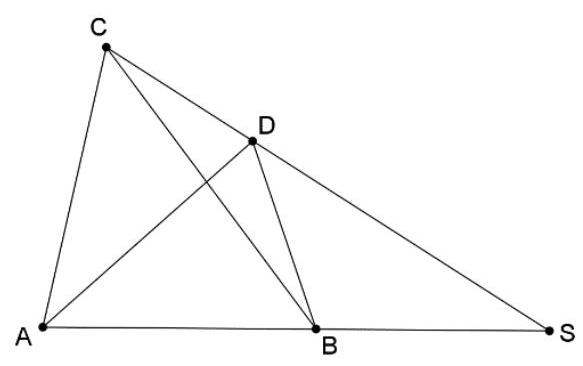
\includegraphics[max width=\textwidth, center]{2024_11_21_8d7e1e416accc1d3f745g-1(1)}\\
2. Niech \(\max \{a, b\}\) oznacza nie mniejszą z liczb \(a, b\), a \(\min \{a, b\}\) oznacza nie większą \(z\) tych liczb. Udowodnij, że dla każdych liczb rzeczywistych \(x, y\) zachodzą równości:\\
а) \(\max \{x, y\}=\frac{x+y+|x-y|}{2}\) oraz\\
b) \(\min \{x, y\}=\frac{x+y-|x-y|}{2}\)\\
3. Znajdź liczbę dziewięciocyfrową utworzoną z cyfr 1, ... , 9 w taki sposób, że każda z tych cyfr występuje dokładnie raz i liczba utworzona z pierwszej cyfry jest podzielna przez 1, liczba utworzona z dwóch pierwszych cyfr jest podzielna przez 2, liczba utworzona z trzech pierwszych cyfr jest podzielna przez 3 itd.

\section*{LICEUM}
\begin{enumerate}
  \item Dany jest trapez \(A B C D\) o podstawach \(A B\) i \(C D\). Punkt E należy do przekątnej \(B D\). Prosta przechodząca przez punkt \(D \mathrm{i}\) równoległa do prostej \(A E\) przecina prostą \(A C\) w punkcie \(F\). Udowodnij, że proste \(B F\) i \(C E\) są równoległe.\\
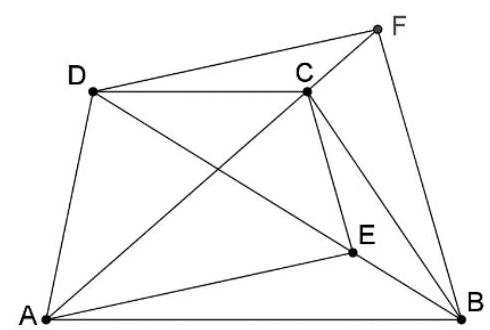
\includegraphics[max width=\textwidth, center]{2024_11_21_8d7e1e416accc1d3f745g-1}
  \item Udowodnij, że dla dowolnych liczb rzeczywistych \(a, b, c\) spełniona jest nierówność
\end{enumerate}

\[
|a+b-c|+|a-b+c|+|-a+b+c| \geq|a|+|b|+|c|
\]

\begin{enumerate}
  \setcounter{enumi}{2}
  \item Udowodnij, że jeśli daną liczbę można przedstawić w postaci sumy kwadratów trzech liczb naturalnych, to jej trzykrotność można zapisać jako sumę kwadratów czterech liczb naturalnych.
\end{enumerate}

\end{document}